\documentclass[12pt,letterpaper]{article}
\usepackage[utf8]{inputenc}
\usepackage[spanish, es-tabla]{babel}
\usepackage[version=3]{mhchem}
\usepackage[journal=jacs]{chemstyle}
\usepackage{amsmath}
\usepackage{amsfonts}
\usepackage{amssymb}
\usepackage{makeidx}
\usepackage{xcolor}
\usepackage[stable]{footmisc}
\usepackage[section]{placeins}
%Paquetes necesarios para tablas
\usepackage{longtable}
\usepackage{array}
\usepackage{xtab}
\usepackage{multirow}
\usepackage{colortab}
%Paquete para el manejo de las unidades
\usepackage{siunitx}
\sisetup{mode=text, output-decimal-marker = {,}, per-mode = symbol, qualifier-mode = phrase, qualifier-phrase = { de }, list-units = brackets, range-units = brackets, range-phrase = --}
\DeclareSIUnit[number-unit-product = \;] \atmosphere{atm}
\DeclareSIUnit[number-unit-product = \;] \pound{lb}
\DeclareSIUnit[number-unit-product = \;] \inch{"}
\DeclareSIUnit[number-unit-product = \;] \foot{ft}
\DeclareSIUnit[number-unit-product = \;] \yard{yd}
\DeclareSIUnit[number-unit-product = \;] \mile{mi}
\DeclareSIUnit[number-unit-product = \;] \pint{pt}
\DeclareSIUnit[number-unit-product = \;] \quart{qt}
\DeclareSIUnit[number-unit-product = \;] \flounce{fl-oz}
\DeclareSIUnit[number-unit-product = \;] \ounce{oz}
\DeclareSIUnit[number-unit-product = \;] \degreeFahrenheit{\SIUnitSymbolDegree F}
\DeclareSIUnit[number-unit-product = \;] \degreeRankine{\SIUnitSymbolDegree R}
\DeclareSIUnit[number-unit-product = \;] \usgallon{galón}
\DeclareSIUnit[number-unit-product = \;] \uma{uma}
\DeclareSIUnit[number-unit-product = \;] \ppm{ppm}
\DeclareSIUnit[number-unit-product = \;] \eqg{eq-g}
\DeclareSIUnit[number-unit-product = \;] \normal{\eqg\per\liter\of{solución}}
\DeclareSIUnit[number-unit-product = \;] \molal{\mole\per\kilo\gram\of{solvente}}
\usepackage{cancel}
%Paquetes necesarios para imágenes, pies de página, etc.
\usepackage{graphicx}
\usepackage{lmodern}
\usepackage{fancyhdr}
\usepackage[left=4cm,right=2cm,top=3cm,bottom=3cm]{geometry}

%Instrucción para evitar la indentación
%\setlength\parindent{0pt}
%Paquete para incluir la bibliografía
\usepackage[backend=bibtex,style=chem-acs,biblabel=dot]{biblatex}
\addbibresource{references.bib}

%Formato del título de las secciones

\usepackage{titlesec}
\usepackage{enumitem}
\titleformat*{\section}{\bfseries\large}
\titleformat*{\subsection}{\bfseries\normalsize}

%Creación del ambiente anexos
\usepackage{float}
\floatstyle{plaintop}
\newfloat{anexo}{thp}{anx}
\floatname{anexo}{Anexo}
\restylefloat{anexo}
\restylefloat{figure}

%Modificación del formato de los captions
\usepackage[margin=10pt,labelfont=bf]{caption}

%Paquete para incluir comentarios
\usepackage{todonotes}

%Paquete para incluir hipervínculos
\usepackage[colorlinks=true,
            linkcolor = blue,
            urlcolor  = blue,
            citecolor = black,
            anchorcolor = blue]{hyperref}

%%%%%%%%%%%%%%%%%%%%%%
%Inicio del documento%
%%%%%%%%%%%%%%%%%%%%%%

\begin{document}
\renewcommand{\labelitemi}{$\checkmark$}

\renewcommand{\CancelColor}{\color{red}}

\newcolumntype{L}[1]{>{\raggedright\let\newline\\\arraybackslash}m{#1}}

\newcolumntype{C}[1]{>{\centering\let\newline\\\arraybackslash}m{#1}}

\newcolumntype{R}[1]{>{\raggedleft\let\newline\\\arraybackslash}m{#1}}

\begin{center}

  \begin{figure}
      \vspace{-45mm}
      \centering
      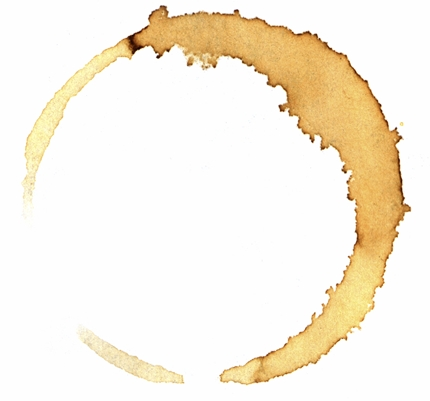
\includegraphics[width=4cm]{./images/cafe-mancha.jpg}
  \end{figure}
  \vspace{-10mm}
  \textbf{\tiny{Apoya tu cafe aqui}} \\
	\vspace{10mm}
  %%%%%%%%%%%%%%%%%%%%%%%%%%%%%%%%%%%%%%
  % Ingresa el mejor titulo que se te ocurra
  %%%%%%%%%%%%%%%%%%%%%%%%%%%%%%%%%%%%%%
	\textbf{\LARGE{Crean Bio Superordenador energéticamente eficiente y obtiene su energía igual que las células vivas. }}\\
	\vspace{4mm}
		\textbf{\large{Tomás Vera\\
  email: \href{mailto:vtomasv@gmail.com}{vtomasv@gmail.com}  } }\\
	\vspace{3mm}
	\textbf{\large{Universidad de Chile}}\\
	\textbf{\small{CC71T-1 Investigación en Cs. de la Computación.(Métodos,Técnicas,Persp.) }}\\
	\textbf{\large{Profesor: Claudio Gutierrez \\
  email: \href{mailto:cgutierr@dcc.uchile.cl}{cgutierr@dcc.uchile.cl}  } }\\
	\today
\end{center}

%%%%%%%%%%%%%%%%%%%%%%%%%%%%%%%%%%%%%%
% Resumen formal de la noticia
%%%%%%%%%%%%%%%%%%%%%%%%%%%%%%%%%%%%%%
\section*{\centering Resumen}
Actualmente controlar la temperatura de los computadores no es una tarea sencilla\autocite{web:1}\autocite{web:2}\autocite{web:3}, adicionalmente se realizan muchos esfuerzos para reducir su consumo energético\autocite{web:4}. Gracias a los avances del profesor Dan Nicolau y su hijo, hoy existe la posibilidad de desarrollar bio-computadores que sean mas eficientes energéticamente, lo que hace que emitan mucho menos calor que los computadores tradicionales.
La investigación llevada a cabo por más de 7 años por los Nicolau (padre e hijo) permitió construir un modelo de computadora biológica que obtiene su energía del trifosfato de adenosina (ATP)\autocite{web:5}, al igual que los hacen las células vivas. Este modelo permite realizar operaciones complejas de la misma manera que los hacen las super computadoras, utilizando procesamiento paralelo.
Las pruebas actuales permitieron construir un chip de 1,5 centímetros cuadrados, que parecen el mapa de una gran ciudad vista desde un avión, sin embargo este chip es capaz de realizar operaciones muy complejas solo usando ATP.
Es importante continuar en la exploración de modelos de esta naturaleza ya que se debe construir un equipo funcional a escala completa, como indica Nicolau \autocite{web:6}. <<Es difícil decir cuándo veremos un bio-superordenador a escala completa. Una de las opciones para hacer frente a problemas más grandes y complejos puede ser combinar nuestro dispositivo con un ordenador convencional para que forme un dispositivo híbrido. En este momento estamos trabajando en una variedad de maneras de llevar la investigación más lejos >>. 


%%%%%%%%%%%%%%%%%%%%%%%%%%%%%%%%%%%%%%
% Tu voz sobre el impacto de esta noticia
%%%%%%%%%%%%%%%%%%%%%%%%%%%%%%%%%%%%%%
\section{Opinion}
El uso de bio computadores significa un salto muy importante, permitiendo la construcción de dispositivos híbridos, llevando uno de los puntos de la computacion atributos de la ciencia de la computación (pasar de lo físico a lo virtual y viceversa ) a otro nivel. Con respecto a los aspectos de ahorro de energía y menor dispersión de calor pueden significar adelantos nunca sospechados, seria muy importante que estos computadores biológicos sean lo mas eficientes posibles y ademas no generen problemas con temperaturas como por ejemplo muchos de nosotros puede observar en los celulares o computadores portátiles.

%%%%%%%%%%%%%%%%%%%%%%%%%%%%%%%%%%%%%%
% Referencias sobre la noticia
%%%%%%%%%%%%%%%%%%%%%%%%%%%%%%%%%%%%%%
\section{Referencias\label{sec:references}}

\printbibliography[heading=none]


\section{Tu opinion es muy importante!}
\begin{figure}
    \centering
    
\includegraphics[width=4cm]{./images/vote.png}
    \captionsetup{justification=centering, singlelinecheck=false}
\end{figure}

\end{document}
